 % $Header: /cvsroot/latex-beamer/latex-beamer/solutions/generic-talks/generic-ornate-15min-45min.en.tex,v 1.5 2007/01/28 20:48:23 tantau Exp $

\documentclass[letter,graphicx]{beamer}

% This file is a solution template for:

% - Giving a talk on some subject.
% - The talk is between 15min and 45min long.
% - Style is ornate.



% Copyright 2004 by Till Tantau <tantau@users.sourceforge.net>.
%
% In principle, this file can be redistributed and/or modified under
% the terms of the GNU Public License, version 2.
%
% However, this file is supposed to be a template to be modified
% for your own needs. For this reason, if you use this file as a
% template and not specifically distribute it as part of a another
% package/program, I grant the extra permission to freely copy and
% modify this file as you see fit and even to delete this copyright
% notice. 



%%%%%%%%%%%%%%%%%%%%%




%%%%%%%%%%%%%%%%%%%%
\mode<presentation>
{
  \usetheme{Warsaw}
  % or ...

  \setbeamercovered{transparent}
  % or whatever (possibly just delete it)
}


\usepackage[english]{babel}
% or whatever

\usepackage[latin1]{inputenc}
% or whatever
\usepackage{verbatim}
\usepackage{times}
\usepackage[T1]{fontenc}
\usepackage{natbib}

\usepackage{xcolor}
\usepackage{tikz}
\usetikzlibrary{shapes.geometric, arrows}

\newcommand{\kid}{\mathrm{kid}}
\newcommand{\ma}{\mathrm{ma}}
\newcommand{\pa}{\mathrm{pa}}
\newcommand{\allelezero}{\tikz\draw[black,fill=white] (0,0) circle (0.8ex);}
\newcommand{\alleleone}{\tikz\draw[black,fill=black] (0,0) circle (0.8ex);}

% here are some tikz definitions
\tikzstyle{pa} = [rectangle, minimum width=0.93cm, minimum height=0.93cm,text centered, draw=black, fill=white]
\tikzstyle{ma} = [circle, minimum width=1cm, text centered, draw=black, fill=white]
\tikzstyle{opa} = [rectangle, minimum width=0.93cm, minimum height=0.93cm, text centered, draw=black, fill=lightgray]
\tikzstyle{oma} = [circle, minimum width=1cm, text centered, draw=black, fill=lightgray]

\tikzstyle{bpa} = [rectangle, minimum width=0.93cm, minimum height=0.93cm, text centered, draw=black, fill=blue!40]
\tikzstyle{bma} = [circle, minimum width=1cm, text centered, draw=black, fill=blue!40]
\tikzstyle{rma} = [circle, minimum width=1cm, text centered, draw=black, fill=red!40]


\tikzstyle{snode} = [circle, minimum width=0.45cm, text centered, draw=black, fill=white] % small node

\tikzstyle{arrow} = [thick,->,>=stealth]



\renewcommand{\bibsection}{\subsubsection*{\bibname } }  % so we don't get a new section!!

%\renewcommand{\citeN}{\shortciteN}
% Or whatever. Note that the encoding and the font should match. If T1
% does not look nice, try deleting the line with the fontenc.

\logo{\includegraphics[width=.1\textwidth]{./images/official_NOAA_logo.pdf}}


% here are some colors for the three different kinds of factors:
\definecolor{pcolor}{rgb}{0,0,1}
\definecolor{gcolor}{rgb}{1, 0.6157, 0}
\definecolor{mcolor}{rgb}{0.89411765, 0.03137255, 0.98039216}

\title[Graphs in Statistics] % (optional, use only with long paper titles)
{Applications of graphs in Statistical\\ 
and Probabilistic Inference}

\subtitle{} % (optional)

\author[Eric C. Anderson] % (optional, use only with lots of authors)
{Eric C.~Anderson}
% - Use the \inst{?} command only if the authors have different
%   affiliation.

\institute[NOAA Fisheries] % (optional, but mostly needed)
{
Fisheries Ecology Division \\ Southwest Fisheries Science Center \\ Santa Cruz, CA \\ USA
}
% - Use the \inst command only if there are several affiliations.
% - Keep it simple, no one is interested in your street address.

\date[Math 115] % (optional)
{
{\footnotesize Guest lecture in Richard Montgomery's course \\
UCSC Math 115, Graph Theory} \\ 
24 February 2016}

\subject{Talks}
% This is only inserted into the PDF information catalog. Can be left
% out. 



% If you have a file called "university-logo-filename.xxx", where xxx
% is a graphic format that can be processed by latex or pdflatex,
% resp., then you can add a logo as follows:

% \pgfdeclareimage[height=0.5cm]{university-logo}{university-logo-filename}
% \logo{\pgfuseimage{university-logo}}



% Delete this, if you do not want the table of contents to pop up at
% the beginning of each subsection:
%\AtBeginSection[]
%{
%  \begin{frame}<beamer>{Outline}
%    \tableofcontents[currentsection,currentsubsection]
%  \end{frame}
%}



% If you wish to uncover everything in a step-wise fashion, uncomment
% the following command: 

%\beamerdefaultoverlayspecification{<+->}

%% More eric commands for inserting some small figures
\newcommand{\smikid}{\includegraphics[width=3.7ex]{images/smiley_blue_kid.pdf}}
\newcommand{\smired}{\includegraphics[width=2.9ex]{images/smiley_sad_red.png}}
\newcommand{\smiblue}{\includegraphics[width=2.9ex]{images/smiley_happy_blue.png}}
\newcommand{\thh}{^\mathrm{th}}
\newcommand{\tc}{\textcolor}
\def\bm#1{\mathpalette\bmstyle{#1}}
\def\bmstyle#1#2{\mbox{\boldmath$#1#2$}}


\begin{document}




\begin{frame}
  \titlepage
\end{frame}



\begin{frame}{Overview}
\begin{itemize}
\item Genetics and pedigrees
\item DAGs, factorization, the idea of inference
\item Undirected graphs (brief)
\item Factor graphs and the sum-product algorithm
\item Inference of pedigrees (brief)
\end{itemize}
\end{frame}






% \subsection{What our data look like}
% %% FLUIDIGM SLIDE
% \begin{frame}{Fluidigm genotyping technology}
% \vspace*{-1.5em}
% \begin{center}
% \mbox{}\hspace*{-.10\textwidth}
% \includegraphics[width=1.16\textwidth]{images/fluidigm.png}
% \end{center}
% $\bullet$ Data: 96 biallelic SNPs (assume unlinked) in 10's of 1,000's of candidate parents and 10's of 1,000's of candidate offspring \\
% $\bullet$ Genotyping error $\leq 1\%$ per locus, but must be addressed.
% \end{frame}

\begin{frame}{Genotype nomenclature and probabilities}
\begin{itemize}
\item AA = \allelezero\,\allelezero{} = 0
\item AG or GA =  \allelezero\,\alleleone{} or \alleleone\,\allelezero{} = 1
\item GG = \alleleone\,\alleleone{} = 2
\end{itemize}
\begin{eqnarray*}
P(Y = 0) & = & (1-q)^2 \\
P(Y = 1) & = & 2q(1-q) \\
P(Y = 2) & = & q^2 \\
\end{eqnarray*}

\end{frame}


\begin{frame}{Simple 3-person pedigree}
\begin{center}
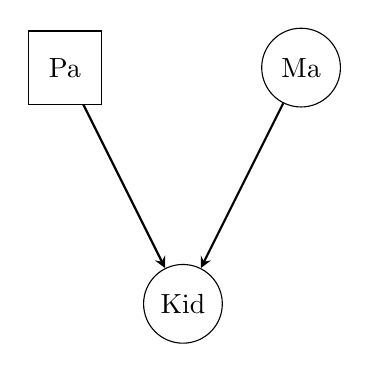
\begin{tikzpicture}[node distance=3cm]

\node (pa) [pa] {Pa};
\node (ma) [ma, right of=pa] {Ma};
\node (kid) [ma, yshift= -3.0cm, xshift=1.5cm] {Kid};

\draw [arrow] (pa) -- (kid);
\draw [arrow] (ma) -- (kid);
\end{tikzpicture}
\end{center}

\end{frame}



\begin{frame}{Conditional probabilities of inheritance}
\mbox{}

{
\renewcommand{\baselinestretch}{1.57}
\small
\[
P(Y_\kid | Y_\pa = 1\;\allelezero\,\alleleone{}, Y_\ma) = \bordermatrix{ 
Y_\kid\downarrow ~ ~ Y_\ma\rightarrow &  0\;\allelezero\,\allelezero{} & 1\;\allelezero\,\alleleone{} & 2\;\alleleone\,\alleleone{} \cr
0\;\allelezero\,\allelezero{}  &  \frac{1}{2}   &  \frac{1}{4}   &  0  \cr
1\;\allelezero\,\alleleone{}   &  \frac{1}{2}   &  \frac{1}{2}   &  \frac{1}{2}  \cr
2\;\alleleone\,\alleleone{}    &     0          &  \frac{1}{4}   &  \frac{1}{2}  \cr
}
\]
}
\renewcommand{\baselinestretch}{1.00}

\end{frame}



\begin{frame}{Computing joint probabilities}

\begin{center}
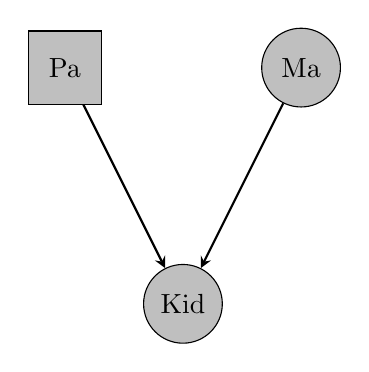
\begin{tikzpicture}[node distance=3cm]

\node (pa) [opa] {Pa};
\node (ma) [oma, right of=pa] {Ma};
\node (kid) [oma, yshift= -3.0cm, xshift=1.5cm] {Kid};

\draw [arrow] (pa) -- (kid);
\draw [arrow] (ma) -- (kid);
\end{tikzpicture}
~~~~~~
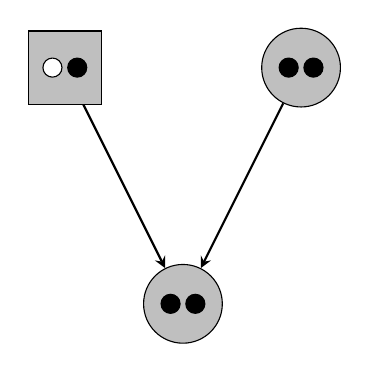
\begin{tikzpicture}[node distance=3cm]

\node (pa) [opa] {\allelezero\,\alleleone};
\node (ma) [oma, right of=pa] {\alleleone\,\alleleone};
\node (kid) [oma, yshift= -3.0cm, xshift=1.5cm] {\alleleone\,\alleleone};

\draw [arrow] (pa) -- (kid);
\draw [arrow] (ma) -- (kid);
\end{tikzpicture}
\end{center}

\end{frame}



\begin{frame}{Inference, a simple example}
Imagine that you have observed the genotype of Pa and Kid, but not Ma,
\begin{center}
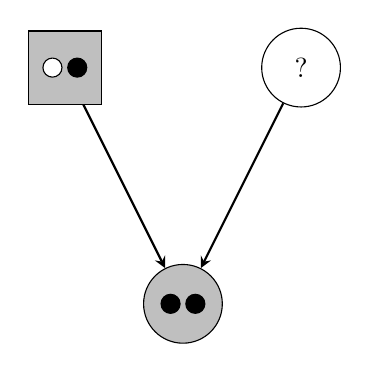
\begin{tikzpicture}[node distance=3cm]

\node (pa) [opa] {\allelezero\,\alleleone};
\node (ma) [ma, right of=pa] {?};
\node (kid) [oma, yshift= -3.0cm, xshift=1.5cm] {\alleleone\,\alleleone};

\draw [arrow] (pa) -- (kid);
\draw [arrow] (ma) -- (kid);
\end{tikzpicture}
\end{center}
\ldots so you would like to use all the information in the above figure to {\em infer} (as best you can)
the genotype of Ma.
\end{frame}






\begin{frame}{A DAG that is not a pedigree}
\begin{center}
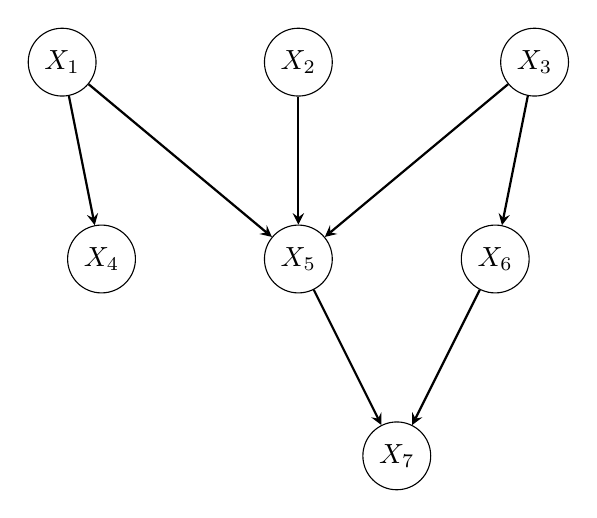
\begin{tikzpicture}[node distance=3cm]

\node (x1) [snode] {$X_1$};
\node (x2) [snode, right of=x1] {$X_2$};
\node (x3) [snode, right of=x2] {$X_3$};
\node (x4) [snode, yshift= -2.5cm, xshift=0.5cm] {$X_4$};
\node (x5) [snode, yshift= -2.5cm, xshift=3.0cm] {$X_5$};
\node (x6) [snode, yshift= -2.5cm, xshift=5.5cm] {$X_6$};
\node (x7) [snode, yshift= -5.0cm, xshift=4.25cm] {$X_7$};

\draw [arrow] (x1) -- (x4);
\draw [arrow] (x1) -- (x5);
\draw [arrow] (x2) -- (x5);
\draw [arrow] (x3) -- (x5);
\draw [arrow] (x3) -- (x6);
\draw [arrow] (x5) -- (x7);
\draw [arrow] (x6) -- (x7);
\end{tikzpicture}
\end{center}
Writing down the factorization of a distribution that respects the above graph is left
as an exercise.
\end{frame}





\begin{frame}{Which relatives really matter?}
Imagine you wish to infer $Y_A$ given everyone in the pedigree.  Whose
genotypes can you ignore?
\begin{center}
\resizebox{!}{0.7\textheight}{
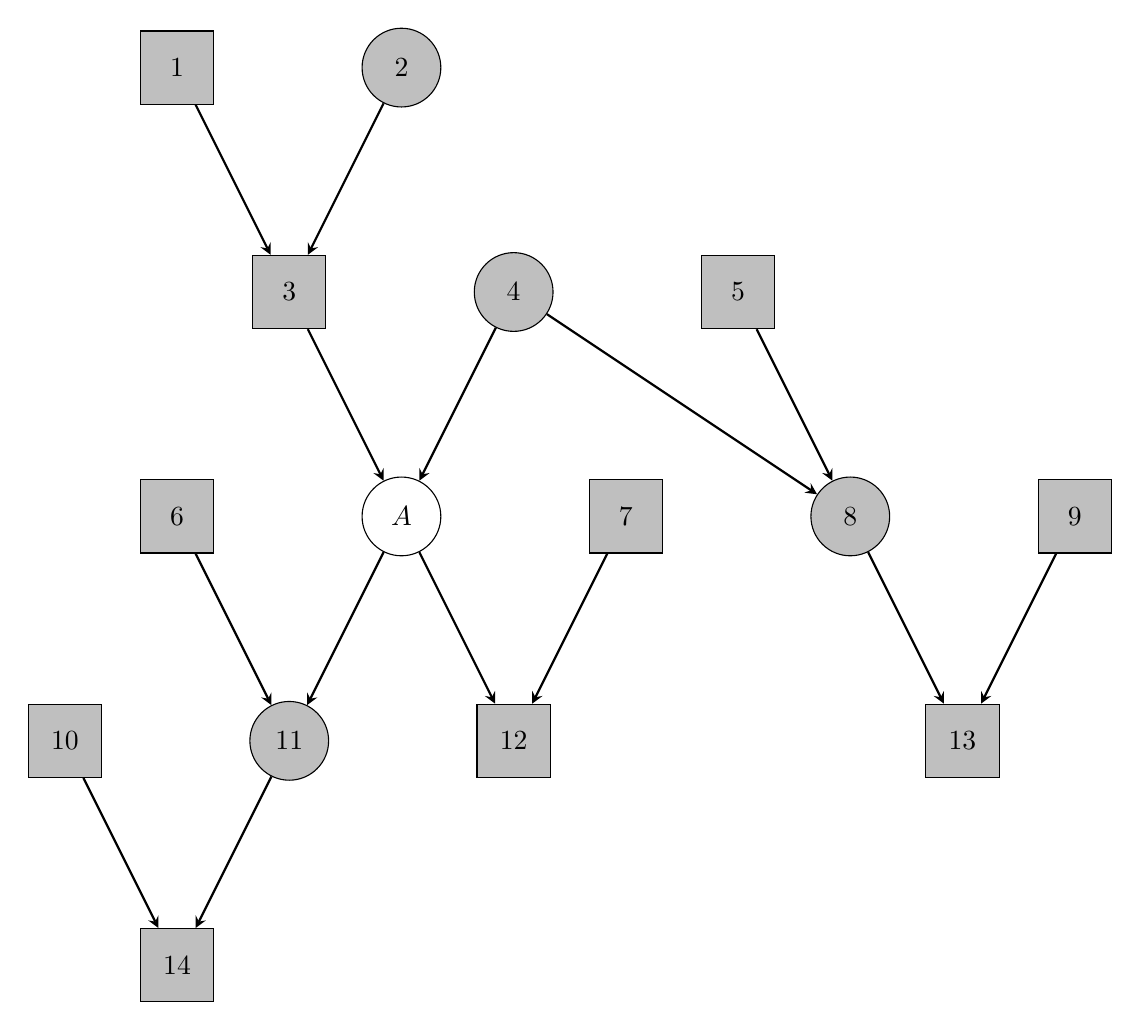
\begin{tikzpicture}[node distance=2.85cm]

\node (1) [opa] {1};
\node (2) [oma, right of=1] {2};

\node (3) [opa, below of=1, xshift=1.425cm] {3};
\node (4) [oma, right of=3] {4};
\node (5) [opa, right of=4] {5};

\node (6) [opa, below of=3, xshift=-1.425cm] {6};
\node (A) [ma, right of=6] {$A$};
\node (7) [opa, right of=A] {7};
\node (8) [oma, right of=7] {8};
\node (9) [opa, right of=8] {9};

\node (10) [opa, below of=6, xshift=-1.425cm] {10};
\node (11) [oma, right of=10] {11};
\node (12) [opa, right of=11] {12};
\node (13) [opa, right of=12, xshift=2.85cm] {13};

\node (14) [opa, below of=10, xshift=1.425cm] {14};

\draw [arrow] (1) -- (3);
\draw [arrow] (2) -- (3);

\draw [arrow] (3) -- (A);
\draw [arrow] (4) -- (A);
\draw [arrow] (4) -- (8);
\draw [arrow] (5) -- (8);

\draw [arrow] (6) -- (11);
\draw [arrow] (A) -- (11);
\draw [arrow] (A) -- (12);
\draw [arrow] (7) -- (12);
\draw [arrow] (8) -- (13);
\draw [arrow] (9) -- (13);

\draw [arrow] (10) -- (14);
\draw [arrow] (11) -- (14);

\end{tikzpicture}
}
\end{center}

\end{frame}








\begin{frame}{Which relatives really matter?}
Look at who $A$ is muddled up with in the terms of the joint probability:
\begin{eqnarray*}
P(\mathrm{all}) & = & P(Y_1)P(Y_2)P(Y_3|Y_1,Y_2)P(Y_4)P(Y_5) \\
  & \times  & P(Y_6)\textcolor{blue}{P(Y_A|Y_3,Y_4)}P(Y_7)P(Y_8|Y_4,Y_5)P(Y_9) \\
  & \times  & P(Y_{10})\textcolor{blue}{P(Y_{11}|Y_6,Y_A)P(Y_{12}|Y_A,Y_7)}P(Y_{13}|Y_8,Y_9) \\
  & \times  & P(Y_{14}|Y_{10},Y_{11})
\end{eqnarray*}

They are \textcolor{blue}{$(Y_3, Y_4, Y_6, Y_7, Y_{11}, Y_{12})$}.
\end{frame}











\begin{frame}{Which relatives really matter?}
Behold! The
relevant relatives are {\em not} all adjacent to $A$ in the directed graph.
\begin{center}
\resizebox{!}{0.7\textheight}{
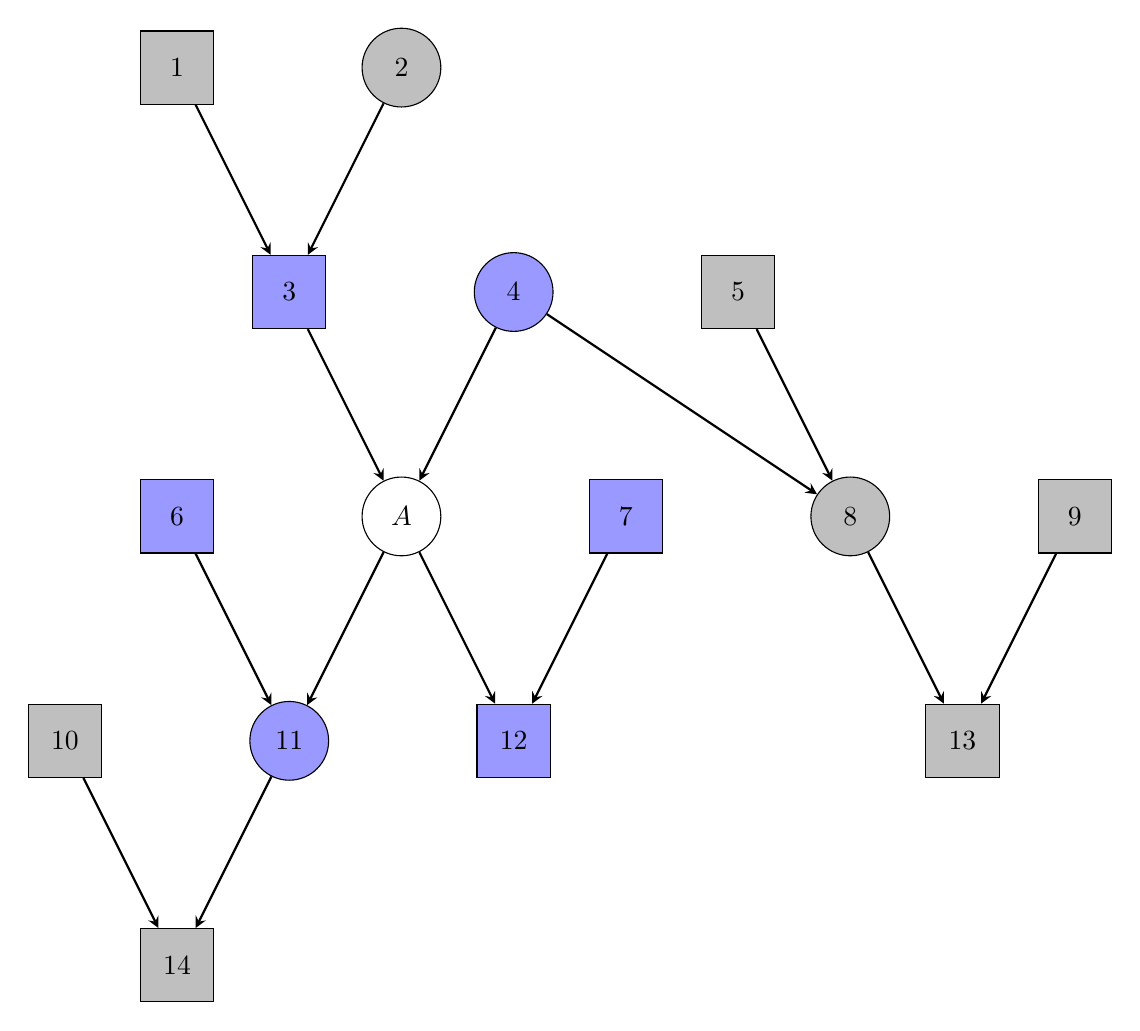
\begin{tikzpicture}[node distance=2.85cm]

\node (1) [opa] {1};
\node (2) [oma, right of=1] {2};

\node (3) [bpa, below of=1, xshift=1.425cm] {3};
\node (4) [bma, right of=3] {4};
\node (5) [opa, right of=4] {5};

\node (6) [bpa, below of=3, xshift=-1.425cm] {6};
\node (A) [ma, right of=6] {$A$};
\node (7) [bpa, right of=A] {7};
\node (8) [oma, right of=7] {8};
\node (9) [opa, right of=8] {9};

\node (10) [opa, below of=6, xshift=-1.425cm] {10};
\node (11) [bma, right of=10] {11};
\node (12) [bpa, right of=11] {12};
\node (13) [opa, right of=12, xshift=2.85cm] {13};

\node (14) [opa, below of=10, xshift=1.425cm] {14};

\draw [arrow] (1) -- (3);
\draw [arrow] (2) -- (3);

\draw [arrow] (3) -- (A);
\draw [arrow] (4) -- (A);
\draw [arrow] (4) -- (8);
\draw [arrow] (5) -- (8);

\draw [arrow] (6) -- (11);
\draw [arrow] (A) -- (11);
\draw [arrow] (A) -- (12);
\draw [arrow] (7) -- (12);
\draw [arrow] (8) -- (13);
\draw [arrow] (9) -- (13);

\draw [arrow] (10) -- (14);
\draw [arrow] (11) -- (14);

\end{tikzpicture}

}
\end{center}
$\bullet$ Is this a moral question?
\end{frame}










\begin{frame}{These are the people in your neighborhood}
The {\em moralized undirected graph} associated with the DAG represents
the {\em Markov blanket} of a vertex via adjacency.
\begin{center}
\resizebox{!}{0.7\textheight}{
\tikzstyle{arrow} = [thick]
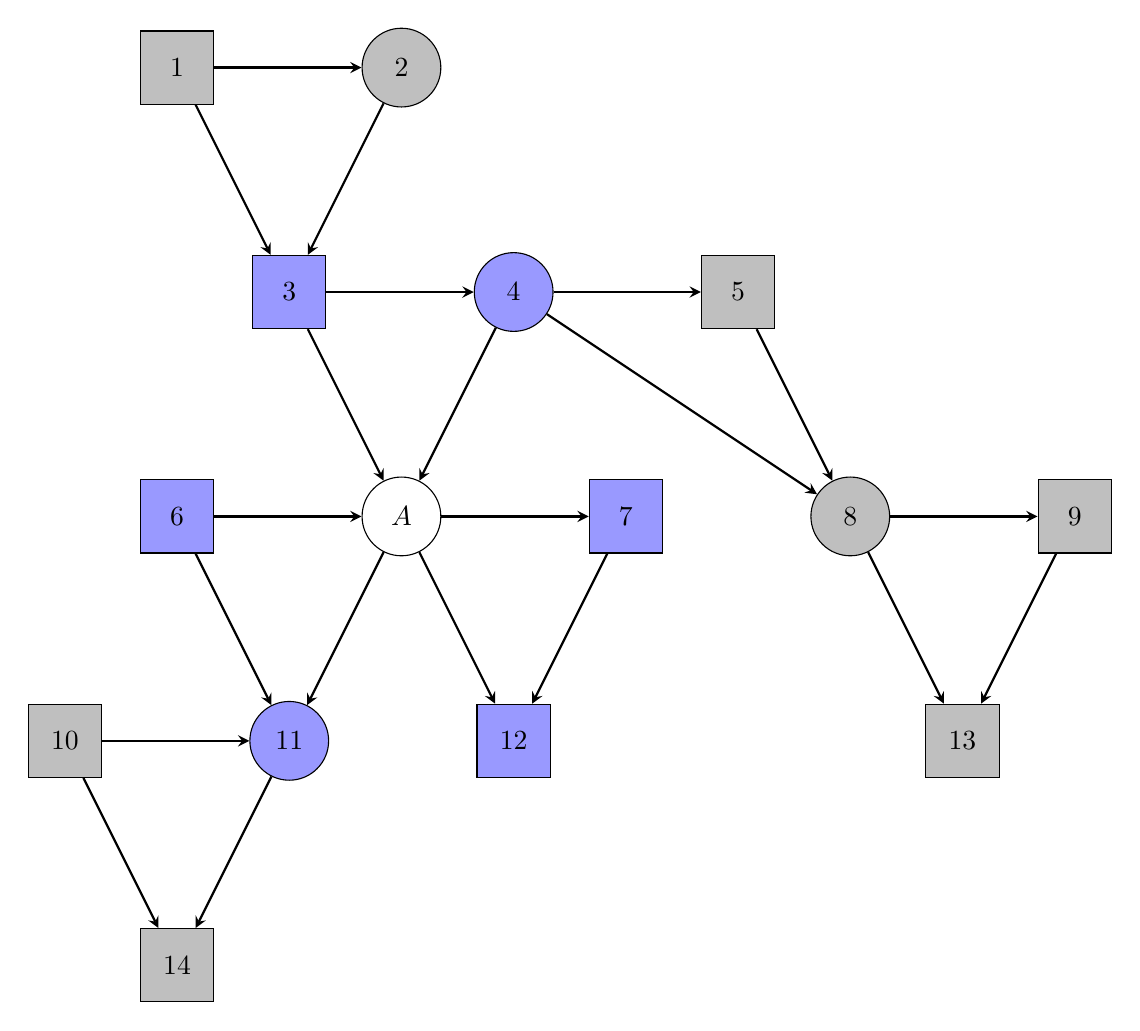
\begin{tikzpicture}[node distance=2.85cm]


\node (1) [opa] {1};
\node (2) [oma, right of=1] {2};

\node (3) [bpa, below of=1, xshift=1.425cm] {3};
\node (4) [bma, right of=3] {4};
\node (5) [opa, right of=4] {5};

\node (6) [bpa, below of=3, xshift=-1.425cm] {6};
\node (A) [ma, right of=6] {$A$};
\node (7) [bpa, right of=A] {7};
\node (8) [oma, right of=7] {8};
\node (9) [opa, right of=8] {9};

\node (10) [opa, below of=6, xshift=-1.425cm] {10};
\node (11) [bma, right of=10] {11};
\node (12) [bpa, right of=11] {12};
\node (13) [opa, right of=12, xshift=2.85cm] {13};

\node (14) [opa, below of=10, xshift=1.425cm] {14};

\draw [arrow] (1) -- (3);
\draw [arrow] (2) -- (3);

\draw [arrow] (3) -- (A);
\draw [arrow] (4) -- (A);
\draw [arrow] (4) -- (8);
\draw [arrow] (5) -- (8);

\draw [arrow] (6) -- (11);
\draw [arrow] (A) -- (11);
\draw [arrow] (A) -- (12);
\draw [arrow] (7) -- (12);
\draw [arrow] (8) -- (13);
\draw [arrow] (9) -- (13);

\draw [arrow] (10) -- (14);
\draw [arrow] (11) -- (14);

\draw [arrow] (1) -- (2);
\draw [arrow] (3) -- (4);
\draw [arrow] (4) -- (5);
\draw [arrow] (6) -- (A);
\draw [arrow] (A) -- (7);
\draw [arrow] (8) -- (9);
\draw [arrow] (10) -- (11);

\end{tikzpicture}
\tikzstyle{arrow} = [thick,->,>=stealth]
}
\end{center}
\end{frame}










\begin{frame}{Inference with latent variables}

\begin{center}
\resizebox{!}{0.7\textheight}{
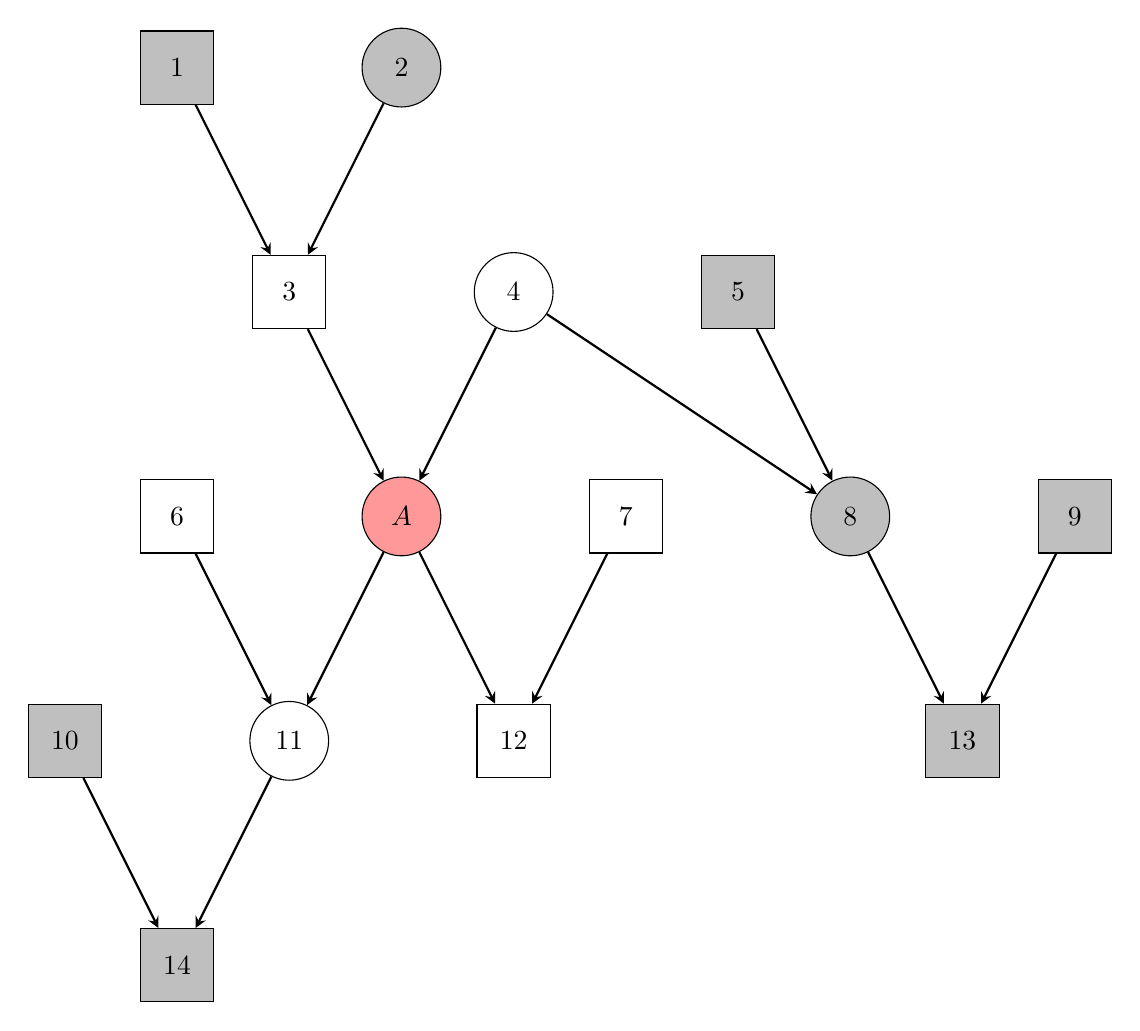
\begin{tikzpicture}[node distance=2.85cm]

\node (1) [opa] {1};
\node (2) [oma, right of=1] {2};

\node (3) [pa, below of=1, xshift=1.425cm] {3};
\node (4) [ma, right of=3] {4};
\node (5) [opa, right of=4] {5};

\node (6) [pa, below of=3, xshift=-1.425cm] {6};
\node (A) [rma, right of=6] {$A$};
\node (7) [pa, right of=A] {7};
\node (8) [oma, right of=7] {8};
\node (9) [opa, right of=8] {9};

\node (10) [opa, below of=6, xshift=-1.425cm] {10};
\node (11) [ma, right of=10] {11};
\node (12) [pa, right of=11] {12};
\node (13) [opa, right of=12, xshift=2.85cm] {13};

\node (14) [opa, below of=10, xshift=1.425cm] {14};

\draw [arrow] (1) -- (3);
\draw [arrow] (2) -- (3);

\draw [arrow] (3) -- (A);
\draw [arrow] (4) -- (A);
\draw [arrow] (4) -- (8);
\draw [arrow] (5) -- (8);

\draw [arrow] (6) -- (11);
\draw [arrow] (A) -- (11);
\draw [arrow] (A) -- (12);
\draw [arrow] (7) -- (12);
\draw [arrow] (8) -- (13);
\draw [arrow] (9) -- (13);

\draw [arrow] (10) -- (14);
\draw [arrow] (11) -- (14);

\end{tikzpicture}
}
\end{center}
How should we go about computing
$P(Y_A|Y_1, Y_2, Y_5, Y_8, Y_9, Y_{10}, Y_{13}, Y_{14})$?

\end{frame}








%% Simple pedigree slide
\begin{frame}{Genetic data on a simple pedigree}

Genotypes $y = (y_1,\ldots, y_{10})$ observed with error, $\epsilon$,  from the true genotypes $x=(x_1,\ldots, x_{10})$. Founders' $x_i$ drawn from allele frequencies $\theta$.

\vspace*{-1em}


\begin{columns}
\column[c]{0.30\textwidth}
\hspace*{-2em}
\includegraphics[width = 1.60\textwidth]{./images/three-gen-ped-basic.pdf}
\column[c]{0.55\textwidth}
\begin{eqnarray*}
 & & p(x,y) = \\
~\\
 &\times &  p(x_1|\theta)p(x_2|\theta)p(x_4|\theta)p(x_5|\theta)  \\
~ \\ 
 & \times& p(x_3|x_1,x_2) p(x_6|x_5,x_4)p(x_7|x_5,x_4)  \\
 & \times& p(x_8|x_3,x_4)p(x_9|x_3,x_4)p(x_{10}|x_3,x_4)  \\
~\\
 & \times& \prod_{i=1}^{10} p(y_i|x_i, \epsilon)
\end{eqnarray*}
\end{columns}
\end{frame}




%% Simple pedigree slide -- Colored equation
\begin{frame}{Genetic data on a simple pedigree}

Genotypes $y = (y_1,\ldots, y_{10})$ observed with error, $\epsilon$,  from the true genotypes $x=(x_1,\ldots, x_{10})$. Founders' $x_i$ drawn from allele frequencies $\theta$.

\vspace*{-1em}

\begin{columns}
\column[c]{0.30\textwidth}
\hspace*{-2em}
\includegraphics[width = 1.60\textwidth]{./images/three-gen-ped-basic.pdf}
\column[c]{0.55\textwidth}
\begin{eqnarray*}
 & & p(x,y) = \\
~\\
 &\times &  \textcolor{pcolor}{p(x_1|\theta)p(x_2|\theta)p(x_4|\theta)p(x_5|\theta)}  \\
~ \\ 
 & \times& \textcolor{mcolor}{p(x_3|x_1,x_2) p(x_6|x_5,x_4)p(x_7|x_5,x_4)}  \\
 & \times& \textcolor{mcolor}{p(x_8|x_3,x_4)p(x_9|x_3,x_4)p(x_{10}|x_3,x_4)}  \\
~\\
 & \times& \textcolor{gcolor}{\prod_{i=1}^{10} p(y_i|x_i, \epsilon)}
\end{eqnarray*}
\end{columns}
\end{frame}



%% Simple pedigree slide -- Colored equations with f's instead of p's
\begin{frame}{Genetic data on a simple pedigree}

These probabilities fall into three different classes of functions of the $x_i$'s: $\textcolor{pcolor}{f_p(x_i)}$, $\textcolor{gcolor}{f_g(x_i)}$, and $\textcolor{mcolor}{f_m(x_\mathrm{pa}, x_\mathrm{ma}, x_{\mathrm{kid},1} \ldots, x_{\mathrm{kid},n})}$, in which $\theta$ and $y$ and $\epsilon$ are implicit (and fixed).  

\vspace*{-1em}

\begin{columns}
\column[c]{0.30\textwidth}
\hspace*{-2em}
\includegraphics[width = 1.60\textwidth]{./images/three-gen-ped-basic.pdf}
\column[c]{0.55\textwidth}
\begin{eqnarray*}
 & & p(x,y) = \\
~\\
 &\times &  \textcolor{pcolor}{f_p(x_1)f_p(x_2)f_p(x_4)f_p(x_5)}  \\
~ \\ 
 & \times& \textcolor{mcolor}{f_m(x_1,x_2,x_3) f_m(x_5,x_4,x_6, x_7)}  \\
 & \times& \textcolor{mcolor}{f_m(x_3,x_4,x_8, x_9, x_{10})}  \\
~\\
 & \times& \textcolor{gcolor}{\prod_{i=1}^{10} f_g(x_i)}
\end{eqnarray*}
\end{columns}
\end{frame}



%% Color Pedigree Factor Graph
\begin{frame}{A factor graph representation}

$p(x,y)$ factorizes into a product over {\em factor nodes} of functions whose arguments
are the adjacent {\em variable nodes}.
\begin{columns}
\column[c]{0.30\textwidth}
\hspace*{-2em}
\includegraphics[width = 1.60\textwidth]{./images/three-gen-basic-factor-color.pdf}
\column[c]{0.55\textwidth}
\begin{eqnarray*}
 & & p(x,y) = \\
~\\
 &\times &  \textcolor{pcolor}{f_p(x_1)f_p(x_2)f_p(x_4)f_p(x_5)}  \\
~ \\ 
 & \times& \textcolor{mcolor}{f_m(x_1,x_2,x_3) f_m(x_5,x_4,x_6, x_7)}  \\
 & \times& \textcolor{mcolor}{f_m(x_3,x_4,x_8, x_9, x_{10})}  \\
~\\
 & \times& \textcolor{gcolor}{\prod_{i=1}^{10} f_g(x_i)}
\end{eqnarray*}
\end{columns}
\end{frame}





%% Sum Product Overview
 \begin{frame}{Sum Product Algorithm on Factor Trees}
 \framesubtitle{\citet{kschischang2001factor} {\em IEEE Transactions on Information Theory}}
 \begin{itemize}
 	\item A message passing algorithm for the (marginal) conditional distribution of each $x_i$ given all the $y_i$'s.
 	\begin{itemize}
 		\item Messages are potential functions of the individual {\em variable nodes} to or from which the messages are being sent.
 		\item Scheduling: a node can send an outgoing message on edge $i$ only when the node has no other edges (apart from $i$) that have {\em not} received an incoming message.
		 \item An outgoing message from variable node $v$ to factor node $t$ on edge $j$ is a simple product of all the incoming messages to $v$ on edges other than $j$.
 		\item An outgoing message from factor node $t$ to variable node $v$ on edge $i$ is the marginal of $v$ given the function associated with $t$ weighted by all incoming messages on edges other than $i$.
 	\end{itemize}
 \end{itemize}
 \end{frame}



%% Bayes theorem via the sum product algorithm
\begin{frame}{Bayes' Theorem via the Sum-Product Algorithm}
\framesubtitle{A single SNP in a single diploid individual}

\begin{columns}
\column[c]{0.25\textwidth}
\includegraphics[height = 0.8\textheight]{./images/single-node-sum-product-a.pdf}
\column[c]{0.55\textwidth}
\begin{itemize}
\item Consider a single SNP with two alleles, 0 and 1, with $p_1 = .4$\\
\item Hence three possible genotypes, 0, 1, and 2, with {\em a priori} 
probability $0.36, 0.48, 0.16$.
\item Observe $y_1 = 2$, but allow a 2\% chance of genotyping error that is equally likely to yield either of the two remaining genotypes, in error.
\end{itemize}
\end{columns}
\end{frame}



%% Bayes theorem via the sum product algorithm -- First round of messages
\begin{frame}{Bayes' Theorem via the Sum-Product Algorithm}
\framesubtitle{Sending the first round of messages}

\begin{columns}
\column[c]{0.25\textwidth}
\includegraphics[height = 0.65\textheight]{./images/single-node-sum-product-b.pdf}
\column[c]{0.55\textwidth}
\begin{itemize}
\item The two factor nodes have only one edge, each\\
\item Hence, they have no other edges with no incoming messages.
\item So, they can send their messages to the variable node.
\end{itemize}
\end{columns}
\end{frame}



%% Bayes theorem via the sum product algorithm -- second round of messages
\begin{frame}{Bayes' Theorem via the Sum-Product Algorithm}
\framesubtitle{Sending the second round of messages}

\begin{columns}
\column[c]{0.25\textwidth}
\includegraphics[height = 0.65\textheight]{./images/single-node-sum-product-c.pdf}
\column[c]{0.55\textwidth}
\begin{itemize}
\item Now,  for each edge connected to the variable node, there are no other edges that have not received incoming messages.
\item Hence the variable node can send outgoing messages on each edge.
\item The message sent is the product of the incoming messages on all the other edges.
\end{itemize}
\end{columns}
\end{frame}





%% Bayes theorem via the sum product algorithm -- using those messages
\begin{frame}{Bayes' Theorem via the Sum-Product Algorithm}
\framesubtitle{Computing quantities using those messages}

\begin{columns}
\column[c]{0.25\textwidth}
\includegraphics[height = 0.45\textheight]{./images/single-node-sum-product-d.pdf}
\column[c]{0.55\textwidth}
\begin{itemize}
\item Each edge has two messages going in different directions.
\item The product of the two messages on an edge connected to a variable node:
\begin{enumerate}
\item Gives the joint probability of $x_i$ and $y$ 
\item Normalizes to the probability of $x_i$ given all the observed data and the allele freq in the population: $\mbox{}\approx (0.02, 0.03, 0.95)$
\end{enumerate}
\end{itemize}
\end{columns}
\end{frame}


%% SP on a sligthly larger pedigre 00
\begin{frame}{Sum-Product Algorithm on a Larger Pedigree}
\begin{center}
\includegraphics[height = 0.8\textheight]{./images/mg-example-step1.pdf}
\end{center}
\end{frame}


\begin{frame}{Sum-Product Algorithm on a Larger Pedigree} 
\begin{center} 
\includegraphics[height = 0.8\textheight]{./images/mg-example-step2.pdf}; 
\end{center}
\end{frame}


\begin{frame}{Sum-Product Algorithm on a Larger Pedigree} 
\begin{center} 
\includegraphics[height = 0.8\textheight]{./images/mg-example-step3.pdf}; 
\end{center}
\end{frame}


\begin{frame}{Sum-Product Algorithm on a Larger Pedigree} 
\begin{center} 
\includegraphics[height = 0.8\textheight]{./images/mg-example-step4.pdf}; 
\end{center}
\end{frame}


\begin{frame}{Sum-Product Algorithm on a Larger Pedigree} 
\begin{center} 
\includegraphics[height = 0.8\textheight]{./images/mg-example-step5.pdf}; 
\end{center}
\end{frame}


\begin{frame}{Sum-Product Algorithm on a Larger Pedigree} 
\begin{center} 
\includegraphics[height = 0.8\textheight]{./images/mg-example-step6.pdf}; 
\end{center}
\end{frame}


\begin{frame}{Sum-Product Algorithm on a Larger Pedigree} 
\begin{center} 
\includegraphics[height = 0.8\textheight]{./images/mg-example-step7.pdf}; 
\end{center}
\end{frame}


\begin{frame}{Sum-Product Algorithm on a Larger Pedigree} 
\begin{center} 
\includegraphics[height = 0.8\textheight]{./images/mg-example-step8.pdf}; 
\end{center}
\end{frame}


\begin{frame}{Sum-Product Algorithm on a Larger Pedigree} 
\begin{center} 
\includegraphics[height = 0.8\textheight]{./images/mg-example-step9.pdf}; 
\end{center}
\end{frame}


\begin{frame}{Sum-Product Algorithm on a Larger Pedigree} 
\begin{center} 
\includegraphics[height = 0.8\textheight]{./images/mg-example-step10.pdf}; 
\end{center}
\end{frame}


\begin{frame}{Sum-Product Algorithm on a Larger Pedigree} 
\begin{center} 
\includegraphics[height = 0.8\textheight]{./images/mg-example-step11.pdf}; 
\end{center}
\end{frame}


\begin{frame}{Sum-Product Algorithm on a Larger Pedigree} 
\begin{center} 
\includegraphics[height = 0.8\textheight]{./images/mg-example-step12.pdf}; 
\end{center}
\end{frame}



\begin{frame}{References}
\tiny
\bibliography{../biblio/pedfactory}
\bibliographystyle{../biblio/men}

\end{frame}
\end{document}


